\documentclass[fleqn,10pt]{olplainarticle}\usepackage[]{graphicx}\usepackage[]{color}
% maxwidth is the original width if it is less than linewidth
% otherwise use linewidth (to make sure the graphics do not exceed the margin)
\makeatletter
\def\maxwidth{ %
  \ifdim\Gin@nat@width>\linewidth
    \linewidth
  \else
    \Gin@nat@width
  \fi
}
\makeatother

\definecolor{fgcolor}{rgb}{0.345, 0.345, 0.345}
\newcommand{\hlnum}[1]{\textcolor[rgb]{0.686,0.059,0.569}{#1}}%
\newcommand{\hlstr}[1]{\textcolor[rgb]{0.192,0.494,0.8}{#1}}%
\newcommand{\hlcom}[1]{\textcolor[rgb]{0.678,0.584,0.686}{\textit{#1}}}%
\newcommand{\hlopt}[1]{\textcolor[rgb]{0,0,0}{#1}}%
\newcommand{\hlstd}[1]{\textcolor[rgb]{0.345,0.345,0.345}{#1}}%
\newcommand{\hlkwa}[1]{\textcolor[rgb]{0.161,0.373,0.58}{\textbf{#1}}}%
\newcommand{\hlkwb}[1]{\textcolor[rgb]{0.69,0.353,0.396}{#1}}%
\newcommand{\hlkwc}[1]{\textcolor[rgb]{0.333,0.667,0.333}{#1}}%
\newcommand{\hlkwd}[1]{\textcolor[rgb]{0.737,0.353,0.396}{\textbf{#1}}}%
\let\hlipl\hlkwb

\usepackage{framed}
\makeatletter
\newenvironment{kframe}{%
 \def\at@end@of@kframe{}%
 \ifinner\ifhmode%
  \def\at@end@of@kframe{\end{minipage}}%
  \begin{minipage}{\columnwidth}%
 \fi\fi%
 \def\FrameCommand##1{\hskip\@totalleftmargin \hskip-\fboxsep
 \colorbox{shadecolor}{##1}\hskip-\fboxsep
     % There is no \\@totalrightmargin, so:
     \hskip-\linewidth \hskip-\@totalleftmargin \hskip\columnwidth}%
 \MakeFramed {\advance\hsize-\width
   \@totalleftmargin\z@ \linewidth\hsize
   \@setminipage}}%
 {\par\unskip\endMakeFramed%
 \at@end@of@kframe}
\makeatother

\definecolor{shadecolor}{rgb}{.97, .97, .97}
\definecolor{messagecolor}{rgb}{0, 0, 0}
\definecolor{warningcolor}{rgb}{1, 0, 1}
\definecolor{errorcolor}{rgb}{1, 0, 0}
\newenvironment{knitrout}{}{} % an empty environment to be redefined in TeX

\usepackage{alltt}
% Use option lineno for line numbers 
\usepackage{amssymb}

\title{Mixtures of Partially Linear Models with Monotone Shape Constraints}

\author[1]{Daniel Leibovitz}
\author[2]{Matthias Loffler}
\affil[1]{danleibovitz@gmail.com}
\affil[2]{Address of second author}

\keywords{Mixture Models, Shape Constraints, Isotonic Regression}

\begin{abstract}
Please provide an abstract of no more than 300 words. Your abstract should explain the main contributions of your article, and should not contain any material that is not included in the main text. 
\end{abstract}
\IfFileExists{upquote.sty}{\usepackage{upquote}}{}
\begin{document}

\flushbottom
\maketitle
\thispagestyle{empty}

\section{Introduction}

Thanks for using Overleaf to write your article. Your introduction goes here! Some examples of commonly used commands and features are listed below, to help you get started.

\section{An overview of contributing models}
\subsection{Mixture models}

Guidelines can be included for standard research article sections, such as this one.
\subsection{Partially Linear Models}
\subsection{Isotonic Regression}
\subsection{Past Work in Mixture Models with Monotone Shape Constraints}
Hello


\section{Proposed Model}
\label{sec:examples}

Use section and subsection commands to organize your document. \LaTeX{} handles all the formatting and numbering automatically. Use ref and label commands for cross-references.


\subsection{Model Structure}


\subsection{Model Estimator}

List steps of Algorithm here.

We are given
\begin{itemize}
  \item[]	$x$ — an \(n \times p\) matrix (independent variables with no shape constraint)
  \item[]	$z$ — an \(n \times q\) matrix (independent variables with monotone shape constraint)
  \item[]	$y$ — an \(n \times 1\) matrix (dependent variable)
  \item[]	$k$ — a positive integer representing the number of categories of latent variable L
  \item[] \( \mathcal{L} \) — an \(n \times k\) matrix representing the posterior probability of observation \(i = 1,…,n\) belonging to latent category \(j = 1,...,k\). Additionally, for all \(i = 1,...,n\) and \(j = 1,...,k\), \( \mathcal{L}_{ij} \) is a real number in the range \([0,1]\), and \( \sum_{j=1}^{k} \mathcal{L}_{ij} = 1 \)
\end{itemize}

\begin{enumerate}
  \item For each \( i \) = 1,...n, set the vector \( \mathcal{L}_{i} \) = \( [\mathcal{L}_{i1},...,\mathcal{L}_{ik}] \) as an instance of a multinomial distribution with k=k and n=1. I.e., randomly assign one of the vector elements of \( [\mathcal{L}_{i1}, ..., \mathcal{L}_{ik}] \) to 1 and all other lik to 0, such that each \( \mathcal{L}_{i} = [0,..., 1, ...,0] \) where 1 is at a random index.
  \item In each iteration d until convergence:
    \begin{enumerate}
      \item M-step
        \begin{enumerate}
          \item hello
        \end{enumerate}
      \item E-step
        \begin{enumerate}
          \item goodbye
        \end{enumerate}
    \end{enumerate}
\end{enumerate}

\section{Simulation Study}

Compare to other algorithms here?


\section{Analysis of Life Expectancy Data}



\section{Discussion}

\subsection{Figures and Tables}

Use the table and tabular commands for basic tables --- see Table~\ref{tab:widgets}, for example. You can upload a figure (JPEG, PNG or PDF) using the project menu. To include it in your document, use the includegraphics command as in the code for Figure~\ref{fig:view} below.

\begin{figure}[ht]
\centering
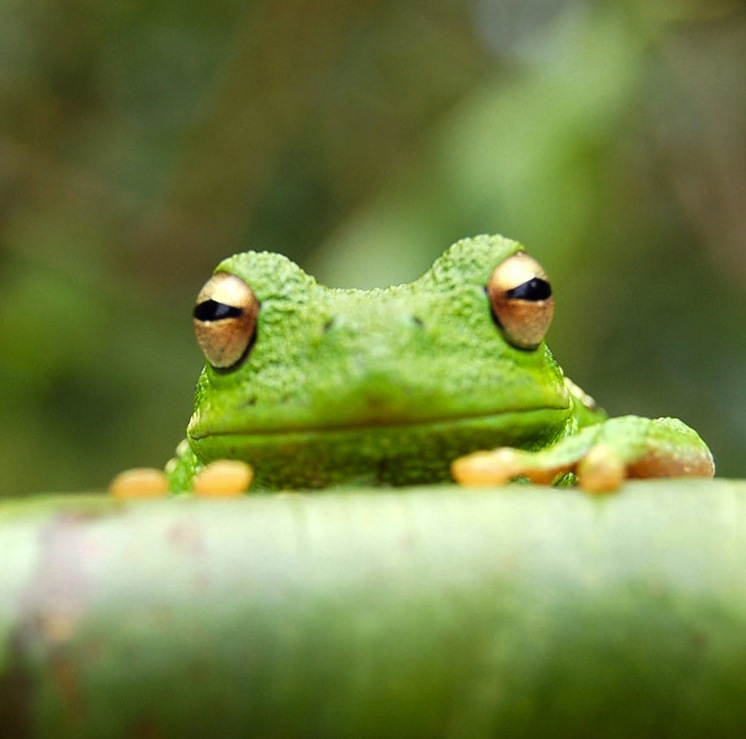
\includegraphics[width=0.7\linewidth]{frog}
\caption{An example image of a frog.}
\label{fig:view}
\end{figure}

\begin{table}[ht]
\centering
\begin{tabular}{l|r}
Item & Quantity \\\hline
Candles & 4 \\
Fork handles & ?  
\end{tabular}
\caption{\label{tab:widgets}An example table.}
\end{table}

\subsection{Citations}

LaTeX formats citations and references automatically using the bibliography records in your .bib file, which you can edit via the project menu. Use the cite command for an inline citation, like \cite{lees2010theoretical}, and the citep command for a citation in parentheses \citep{lees2010theoretical}.

\subsection{Mathematics}

\LaTeX{} is great at typesetting mathematics. Let $X_1, X_2, \ldots, X_n$ be a sequence of independent and identically distributed random variables with $\text{E}[X_i] = \mu$ and $\text{Var}[X_i] = \sigma^2 < \infty$, and let
$$S_n = \frac{X_1 + X_2 + \cdots + X_n}{n}
      = \frac{1}{n}\sum_{i}^{n} X_i$$
denote their mean. Then as $n$ approaches infinity, the random variables $\sqrt{n}(S_n - \mu)$ converge in distribution to a normal $\mathcal{N}(0, \sigma^2)$.

\subsection{Lists}

You can make lists with automatic numbering \dots

\begin{enumerate}[noitemsep] 
\item Like this,
\item and like this.
\end{enumerate}
\dots or bullet points \dots
\begin{itemize}[noitemsep] 
\item Like this,
\item and like this.
\end{itemize}
\dots or with words and descriptions \dots
\begin{description}
\item[Word] Definition
\item[Concept] Explanation
\item[Idea] Text
\end{description}

\section*{Acknowledgments}

Additional information can be given in the template, such as to not include funder information in the acknowledgments section.

\bibliography{sample}

\end{document}
